\chapter{Analysis and methodology}
\label{ana-meth}

\section{Time series forecasting - general model structure}
A model for time series forecasting must be structured in the following way.
As input, it must take a sequence of vectors, with each vector representing a single point in time, and each element of the vector representing an element of the multivariate time series.
For example, a multivariate time series of load and temperature would be represented by a sequence of vectors, each with two elements.
As output, the system must similarly produce a sequence of multivariate vectors.
In the case that the model is forecasting only a single time series, the output vectors will have only a single element each.
This structure is presented in Figure \ref{fig:forecast-model}.
Of course, it may be the case that a time series forecasting model is comprised of several models cascaded together.
Perhaps the sequence of input vectors are concatenated by one model, then passed to the actual forecasting model which produces a single output vector, then the output vector is split by a third model before being produced at the output.

\begin{figure}
	\centering
	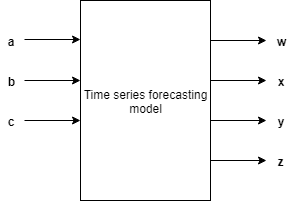
\includegraphics[width=0.35\linewidth]{images/forecast-model}
	\caption{A time series forecasting model takes a sequence of vectors, $\va, \vb, \vc$, as input and produces a sequence of vectors, $\vw, \vx, \vy, \vz$, as output. Note the number of input and output vectors is able to vary.}
	\label{fig:forecast-model}
\end{figure}

This structure - with sequences of input and output vectors - is identical to that used for neural machine translation (NMT), where a source sentence/phrase is translated from one language, say English, to another language such as Dutch \citep{Cho2014}.
In NMT, a word is represented by a vector, and a sentence is represented by a sequence of vectors.

\par
This section will investigate the performance of several of the best performing NMT architectures when applied to time series forecasting.
\hl{I'm still deciding whether I want to put the evaluation before I discuss in detail how the architectures work.
	Benefit of putting evaluation first is that it prevents the reader from being daunted by too much detail upfront.
	Might seem a little backwards though.}

\section{Investigated models and methods}
The following models will be discussed and their results in time series forecasting compared.
\begin{itemize}
	\item ARIMA
	\item Sequence to sequence (S2S) recurrent neural network (RNN) \citep{Cho2014a} using long short term memory (LSTM) \citep{hochreiter1997long} cells
	\item Transformer \citep{Vaswani2017}
	\item Universal Transformer \cite{Dehghani2018}
	\item Clio - a modified transformer with the ability to automatically select similar profile data
\end{itemize}

Additionally, a similar profile selection method was developed to provide the models with relevant input data.
These models and methods are described in the following sections.

\section{ARIMA}
\todo[inline]{todo Change X to Y for output}
\todo[inline]{todo make consistent with Nomenclature chapter}
\par
The ARIMA model is an extension of the autoregressive moving average (ARMA) model, which is comprised of an autoregressive (AR) term and a moving average (MA) term.
\\
Consider a time series $X$, being drawn from some underlying process, with elements $X_{t}, X_{t-1}, ..., X_{0}$. 
\\
An autoregressive model is given by
\begin{equation}
X_{t} = \alpha_{1}X_{t-1} + \alpha_{2}X_{t-2} + \ldots + \alpha_{p}X_{t-p} + \epsilon_{t} = \epsilon_{t} + \sum_{i=1}^{p}\alpha_{i}X_{t-i}
\end{equation}
where $p$ is the order of the AR model, $\alpha$ are the parameters of the model, and $\epsilon_{t}$ is a random normally distributed error with zero mean and variance $\sigma^2$. 
\\ 
A moving average model is given by 
\begin{equation}
X_{t} = \theta_{1}\epsilon_{t-1} + \theta_{2}\epsilon_{t-2} + \ldots + \theta_{q}\epsilon_{t-q} + \epsilon_{t} = \epsilon_{t} + \sum_{i=1}^{q}\theta_{i}\epsilon_{t-i}
\end{equation}
where $q$ is the order of the MA model, $\theta$ are the parameters of the model, and $\epsilon_{t}$ is, again, a random normally distributed error with zero mean and variance $\sigma^2$.
\par
The AR and MA models are combined to form an ARMA model, given by 
\begin{equation}
X_{t} = \epsilon_{t} + \sum_{i=1}^{q}\theta_{i}\epsilon_{t-i} + \sum_{i=1}^{p}\alpha_{i}X_{t-i}
\end{equation}
\par
An ARMA model requires the time series, $X$, being forecast to come from a weakly stationary process.
That is, the mean and autocovariance of the the process do not change with time.
\par
The ARIMA model is an extension to the ARMA model that can be applied when non-stationarity is exhibited by the underlying process.
ARIMA applies differencing to the time series prior to applying the ARMA model to the new time series $\hat{X}$.
This differencing is applied such that $\hat{X}_{t} = X_{t} - X_{t-1}$ and is repeated $d$ times.
Differencing can sometimes be sufficient to make a series stationary, such that it is appropriate for forecasting with an ARMA model.
\par
In order to concisely articulate the ARIMA model, the following notation will be used. The backward shift operator, defined by $\textbf{B}^{m}X_{t} = X_{t-m}$. The difference operator, defined by $\nabla_{s} X_{t} = X_{t} - X_{t-s} = (1 - \textbf{B}^{s})X_{t}$. The parameter functions $\alpha_{p}(\textbf{B}) = 1 - \alpha_{1}\textbf{B} - \ldots - \alpha_{p}\textbf{B}^p$ and $\theta_{q}(\textbf{B}) = 1 + \theta_{1}\textbf{B} + \ldots + \theta_{q}\textbf{B}^q$.
\par
Using this notation, the ARIMA model can be represented as the following
\begin{equation}
\alpha_{p}(\textbf{B})(\nabla_{1}^{d}X_{t}) = \theta_{q}(\textbf{B})\epsilon_{t}
\end{equation}
This is identical to an ARMA model, except that $X_{t}$ has been replaced with a  version of itself, $\nabla_{1}^{d}X_{t}$, that has been differenced $d$ times.
The above model is denoted ARIMA($p,d,q$).
\par
Differencing with a lag of one, as applied by the differencing operator, is not always sufficient to make the series stationary even when performed multiple ($d$) times.
A further extension of the ARIMA model is the seasonal ARIMA (SARIMA) model, which takes into account seasonal patterns which require differencing with a lag greater than one, such as daily, weekly, and yearly seasonalities commonly found in electrical load time series.
\\
Denoted ARIMA$(p,d,q)\times(P,D,Q)s$, a SARIMA model can be represented as the following
\begin{equation}
\alpha_{p}(\textbf{B})A_{P}(\textbf{B}^{s})(\nabla_{1}^{d}\nabla_{s}^{D}X_{t}) = \theta_{q}(\textbf{B})\Theta_{Q}(\textbf{B}^{s})\epsilon_{t}
\end{equation}
Where $(p,d,q)$ are the parameters of the non-seasonal ARIMA component, $(P,Q,D)s$ are the parameters of the seasonal component, $A_{P}(\textbf{B}^{s})$ and $\Theta_{Q}(\textbf{B}^{s})$ are defined similarly to $\alpha_{p}(\textbf{B})$ and $\theta_{q}(\textbf{B})$, and $s$ is the number of periods over which the seasonality occurs (e.g. $s=7$ for weekly seasonality if the data is daily).
\par
The SARIMA model can be further extended to a SARIMA with exogenous variables (SARIMAX) model. 

\section{Recurrent neural network}

\subsection{Generic RNN}
The recurrent neural network RNN architecture was introduced by \cite{Rumelhart1986} in 1986.
RNNs operate on sequences of data by applying an identical function $f$ to every element of the sequence to produce a sequence of state vectors $\vh$.
$f$ takes as input the output of the function at the previous point in the sequence, and the current element of the input sequence $\vx$.
At each point $t$ in the sequence $\vh^t$ is taken as the output.
An RNN can be unfolded to represent it as a traditional feedforward neural network with no recurrence.
A generic RNN is shown in figure \ref{fig:basic_rnn}.

\begin{figure}[htbp]
	\centerline{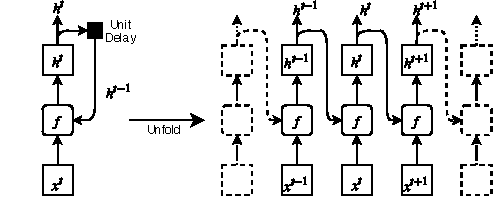
\includegraphics[trim=0 0cm 0 0, width=.5\textwidth]{images/basic_rnn.pdf}}
	\caption{A generic recurrent neural network, operating on an input sequence of $\vx$ vectors and producing an output sequence of $\vh$ vectors.
		     Both the recurrent and unfolded purely feedforward representations are shown.
		     The function $f$ can be replaced with any arbitrary function.}
	\label{fig:basic_rnn}
\end{figure}

RNNs can be extended to multiple layers, with a two-layer RNN illustrated in figure \ref{fig:multilayer_rnn}.
Each layer implements it's own function, with layer $n$ implementing function $f_n$ and producing output $\vh_n$.
For layers after the first layer, instead of taking an $\vx$ vector as input they take the state vector from the previous layer.
There can be an arbitrary number of layers.

\begin{figure}[htbp]
	\centerline{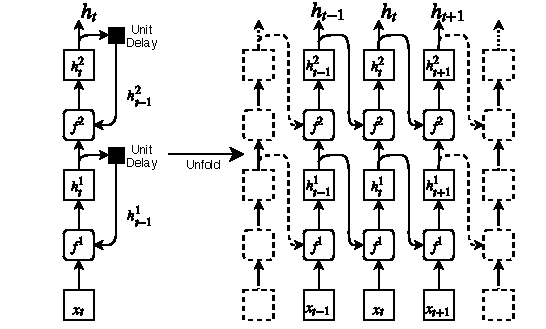
\includegraphics[trim=0 0cm 0 0, width=.5\textwidth]{images/multilayer_rnn.pdf}}
	\caption{A two-layer RNN.}
	\label{fig:multilayer_rnn}
\end{figure}

\subsection{Long short-term memory}
RNNs are prone issues with vanishing and exploding gradients \cite{Goodfellow-et-al-2016}, which is addressed through the use of a long short-term memory (LSTM) \cite{hochreiter1997long} cell as the function in the RNN.
An LSTM cell is able to selectively add and remove elements from the state as it passes through and generally outperforms simpler functions \hl{get some sources}.

\begin{figure}[htbp]
	\centerline{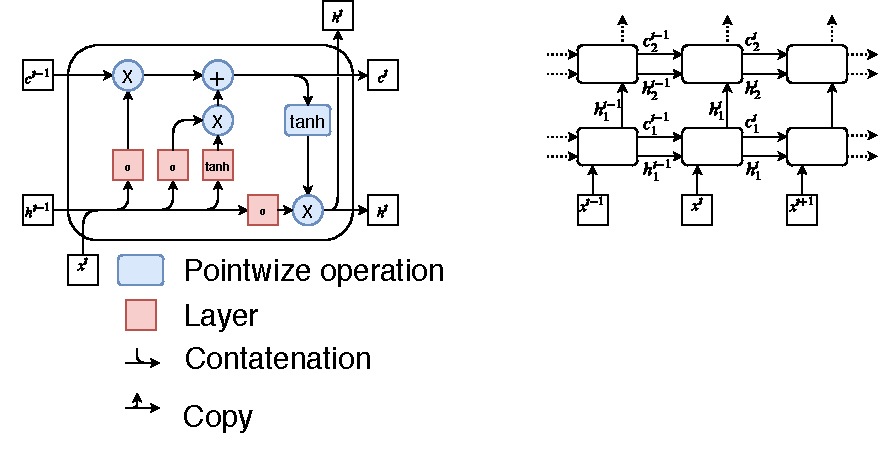
\includegraphics[trim=0 0cm 0 0, width=.65\textwidth]{images/LSTM.pdf}}
	\caption{A LSTM cell and it's configuration in a multilayer RNN.}
	\label{fig:LSTM}
\end{figure}

\subsection{Sequence to sequence}
An RNN can be extended to form a sequence to sequence (S2S) architecture by applying an encoder RNN to an input sequence, and then having a decoder RNN produce an output sequence.
The decoder RNN's initial cell state is set to the final cell state of the encoder \cite{Cho2014a}.
The encoder's final cell state is a latent representation of the input, which is used by the decoder to produce an output.
The encoder and decoder can be of different lengths, allowing this architecture to naturally model tasks such as load forecasting where the input may be 48 hours of data while the output is only 24.

\section{Transformer}
The transformer neural network architecture, shown in figure \ref{fig:transformer}, was introduced by \cite{Vaswani2017} in 2017 and at the time was the state of the art in neural machine translation.
This architecture follows the standard sequence-to-sequence/encoder-decoder architecture: the encoder transforms an input sequence $X = (\boldsymbol{x}_1, ..., \boldsymbol{x}_P)$ into a latent representation $Z = (\boldsymbol{z}_1, ..., \boldsymbol{z}_M)$, and the decoder transforms $Z$ into an output sequence $Y = (\boldsymbol{y}_1, ..., \boldsymbol{y}_R)$, where $x_t$, $y_t$, and $z_t$ are of arbitrary dimension.
This matches the requirements of a load forecasting system, where $P$ is the length of the time series input, $x_t$ is of dimension equal to the number of variables in the input time series, $R$ is the length of the time series output, and $y_t$ is of dimension equal to the number of variables in the output time series.
The latent representation $Z$ is used solely by the model as an internal representation of the input data.

\begin{figure}[htbp]
	\centerline{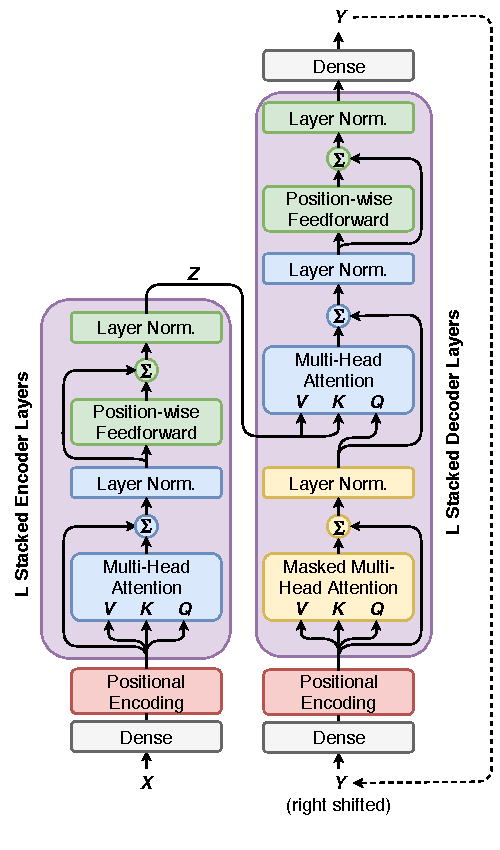
\includegraphics[trim=0 0.8cm 0 0, width=.35\textwidth]{images/transformer.pdf}}
	\caption{The Transformer architecture.}
	\label{fig:transformer}
\end{figure}

The encoder is constructed of a stack of $L$ identical layers, each containing two sub-layers.
The first is multi-head self-attention and the second is a position-wise feed-foward network.
Both sub-layers have a residual connection around them and are fed into a normalization layer.

The decoder is similar to the encoder except for a third layer which implements multi-head attention on the outputs of the encoder.
The input to the decoder is the previous output of the decoder, but shifted right by one.
This requires an iterative approach to be used to predict all points in the time series.
The self-attention in the decoder is masked so that when evaluating a query at time $t$ it does not assign large weights to keys/values occurring after $t$ in time, making the decoder autoregressive.

The individual components of the transformer are discussed in the following sections.

\subsection{Input Embedding}
The input $\boldsymbol{X} \in \mathbb{R}^{T \times N}$, where the rows represent $T$ points in time and the columns represent $N$ time series, is embedded by applying a dense layer to produce an embedded $\boldsymbol{X'} \in \mathbb{R}^{T \times d}$, where $d$ is the hidden dimension of the model and $d$ is the same for both the encoder and the decoder.
This is intended to allow the neural network to learn the relationships and dependencies between the different input time series.
The embedded representation is given by Equation \ref{dense_layer}, with learned weights $\boldsymbol{W} \in \mathbb{R}^{N \times d}$ and a learned bias vector $\boldsymbol{b} \in \mathbb{R}^{d}$.

\begin{equation} \label{dense_layer}
\text{dense}(\boldsymbol{X}) = \text{max}(0, \boldsymbol{XW} + \boldsymbol{b})
\end{equation}

\subsection{Positional Encoding}
The model has no way of telling the position or order of each element in the input, so this information is injected in the positional encoding layer.
This is done by using a learned lookup table to add the same value to the inputs at both test and train time depending on their position in time in the input.
Specifically, the positional encoding layer adds a matrix lookup table of embeddings $\boldsymbol{E}$ to the input, where $\boldsymbol{E}$ is of the same dimension as the input.

\subsection{Multi-Head Attention} \label{multihead_attention}
The primary innovation of the Transformer architecture is multi-head attention.
Generic attention and dot-product attention will now be described as these are prerequisite to describing multi-head attention.

Given a single query vector and a set of key and value pairs (with each key and each value being a vector), an attention function matches the query to the keys to produce a weight for each key by applying an arbitrary fitness function.
These key weights are then used to create an output vector comprised of the weighted sum of the values, where each value's weight is the weight assigned to its corresponding key. 

\begin{figure}[htbp]
	\centerline{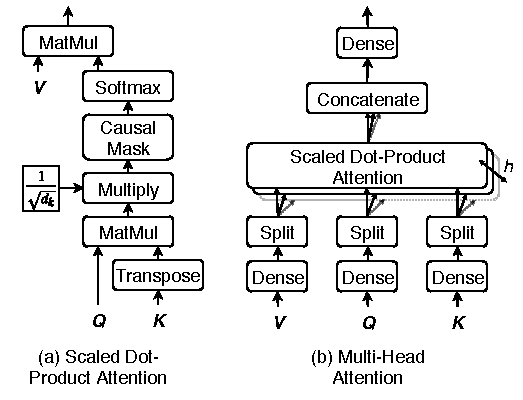
\includegraphics[width=.35\textwidth]{images/multihead_attn.pdf}}
	\caption{Multiheaded attention (b) splits the key, query, and value matrices and applies scaled dot product attention (a) on each in parallel before concatenating the result to return the data to its original dimension.}
	\label{fig:multihead}
\end{figure}

Scaled dot-product attention, shown in Figure \ref{fig:multihead} (a), is a specific implementation of an attention function. 
It uses the dot product of the query and each key to generate the weights, which are then passed through a softmax function such that the sum of all weights is equal to 1.
In practice, the query row vectors are combined into a single matrix, $\boldsymbol{Q}$, allowing cheap matrix calculations to be used to evaluate the attention outputs in parallel.
The keys and values are represented by row vectors in $\boldsymbol{K}$ and $\boldsymbol{V}$, respectively.

The dot product of the keys and queries is scaled (hence the name) by multiplying it by $1 / \sqrt{d_k}$, with $d_k$ being the key and query dimension, to prevent the dot product from becoming large when $d_k$ is large as this may cause the softmax gradient to become very small and affect the gradient descent training.

The causal mask shown in Figure \ref{fig:multihead} is used exclusively in the decoder self-attention to prevent the attention function from matching any query to a key that occurs after itself in time.
This is achieved by leaving the lower triangular portion of the matrix untouched and setting the other values to be large negative numbers, indicating a very poor match.

Multi-head attention, shown in Figure \ref{fig:multihead} (b), applies a separate dense layer to each of the values, queries, and keys. 
The dense layer is applied per Equation \ref{dense_layer} with learned weights $\boldsymbol{W} \in \mathbb{R}^{d \times d}$ and a learned bias vector $\boldsymbol{b} \in \mathbb{R}^{d}$.
The outputs of the dense layers are then split along the last axis into $h$ sets, or heads.
As a result the key, query, and value dimension is reduced by a factor of $h$ to $\frac{d}{h}$.
Scaled dot-product attention is then run independently on each set.
The results are concatenated and put through a final dense layer to produce the output of the attention function.
The dense layer function on the output is defined by Equation \ref{dense_layer} where $\boldsymbol{W} \in \mathbb{R}^{d \times d}$ is a learned weight matrix and $\boldsymbol{b} \in \mathbb{R}^{d}$ is a learned bias vector.

The dense layer combined with the split allows the multi-head attention to pick out information from different subspaces in the input and direct these to different attention heads.
This is in contrast to a single head which must average all subspaces.

\subsection{Feed-forward}
The feed-forward layer is a two layer network with a rectified linear unit in the middle.
Given an input $\boldsymbol{X} \in \mathbb{R}^{T \times d}$, the output $\boldsymbol{X'} \in \mathbb{R}^{T \times d}$ is populated by Equation \ref{feedforward} where $\boldsymbol{W}_1 \in \mathbb{R}^{d \times 4d}$, $\boldsymbol{b}_1 \in \mathbb{R}^{4d}$, $\boldsymbol{W}_2 \in \mathbb{R}^{4d \times d}$, and $\boldsymbol{b}_2 \in \mathbb{R}^{d}$ are learned weights and biases.

\begin{equation} \label{feedforward}
\text{feedforward}(\boldsymbol{X}) = \text{max}(0, \boldsymbol{X}  \boldsymbol{W}_1 + \boldsymbol{b}_1)  \boldsymbol{W}_2 + \boldsymbol{b}_2
\end{equation}

\subsection{Decoder Dense Output}
The output of the decoder is passed through a dense layer to project the hidden dimension to the desired dimension of 1.
The layer is implemented per Equation \ref{dense_layer} where $\boldsymbol{W} \in \mathbb{R}^{d \times 1}$ is a learned weight matrix and $\boldsymbol{b} \in \mathbb{R}^{1}$ is a learned bias vector.
By adjusting the dimension of $\boldsymbol{W}$ and $\boldsymbol{b}$ the network could be modified to perform multiple forecasts simultaneously.


\subsection{Residuals \& Normalization}
Residual connections \cite{He2015} are applied around each sub-layer.
That is, the output of each sub-layer is given by $\boldsymbol{X'} = \boldsymbol{X} + \text{subLayer}(\boldsymbol{X})$ where subLayer$(\boldsymbol{X})$ is the original output of the sub-layer.
The outputs are then normalized by applying layer normalization \cite{Ba2016}, as per Equation \ref{layernorm} where $\mu_{\boldsymbol{x}}$ and $\sigma_{\boldsymbol{x}}$ are the mean and variance of $\boldsymbol{x}$ respectively.

\begin{equation} \label{layernorm}
\boldsymbol{Y}_{i,*} = \frac{\mu_{\boldsymbol{X}_{i,*}}}{\sigma_{\boldsymbol{X}_{i,*}}}
\end{equation}

\subsection{Dropout and Training}
To help prevent overfitting to the training data, dropout \cite{srivastava14a} is applied during training at the output of both positional encoding layers, and immediately after the softmax operation in all multi-head attention layers.

When testing or being used for inference, the decoder outputs are generated sequentially one at a time.
After each output value is generated it is shifted right by one and populated in the decoder input and the model is executed again until all the outputs have been generated.
Values that have not yet been generated are set to zero in the decoder input.
These zero values do not affect the output of the decoder, as the decoder self-attention is masked so that it does not make use of them.
When training, the decoder input is set to the known expected value and the model is executed --- and the learnable parameters updated --- a single time.

\section{Universal Transformer}
Same as transformer, except layers share weights, plus temporal encoding. One page probably.

\section{Clio}

\begin{figure}[htbp]
	\centerline{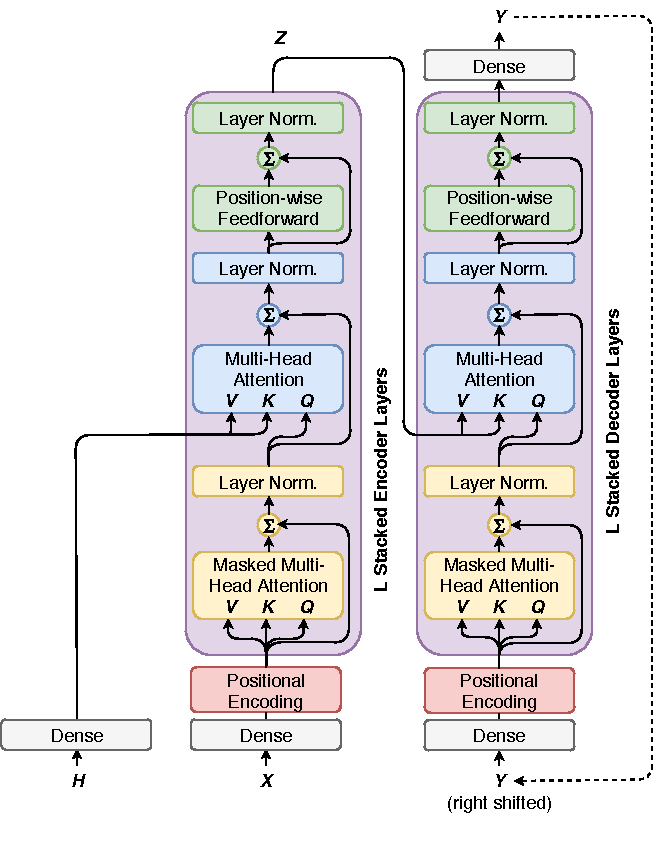
\includegraphics[width=.35\textwidth]{images/clio.pdf}}
	\caption{Clio architecture.}
	\label{fig:clio}
\end{figure}

The Clio architecture is a variation on the Transformer, and is an innovation of this thesis.
In this architecture, an additional multi-head attention layer is employed in the encoder to look over a long sequence of historical data $\mH$ as shown in figure \ref{fig:clio}.

To produce $\mH$, the thirty days of historical data immediately before and after the date of the forecast from every past year is concatenated.
The 30 days prior to the time being forecast is also included.
For example, if a forecast was being performed at 1\textsuperscript{st} June 2018 then data would be concatenated from 1\textsuperscript{st} May 2018 through 1\textsuperscript{st} June 2018, 1\textsuperscript{st} May 2017 through 1\textsuperscript{st} July 2017, 1\textsuperscript{st} May 2016 through 1\textsuperscript{st} July 2016, etc.
For testing and training data is also taken from future years, but never from the 30 days immediately after the date being forecast.
As a result, $\mH \in \mathbb{R}^{T \times h}$ where $T$ is the number of observations and $h$ is the number of variables in each observation.

$\mH$ is embedded by a single dense layer, given by Equation \ref{dense_layer}, with learned weights $\boldsymbol{W} \in \mathbb{R}^{h \times d}$ and a learned bias vector $\boldsymbol{b} \in \mathbb{R}^{d}$.
This reshapes $\mH$ into $\boldsymbol{H'} \in \mathbb{R}^{T \times d}$ to match the hidden dimension of the remainder of the model.

$\mH$ will be very large in practice.
For example, with five years of 30-minute data the embedded $\mH$ will contain around 850e3 elements.
On the other hand, the embedded $\mX$ typically contains around 6e3 elements.
The Clio architecture is an order of magnitude more computationally expensive than the others discussed.


\section{Training and Regularization}
Training and regularization is common to all described models.
The encoder inputs, decoder inputs, and expected outputs were summed with randomly distributed noise with a mean of 0 and standard deviation of 0.01 before being supplied to the model during training.
This has been demonstrated to improve the generalization ability of a neural network \cite{Wang1999} \cite{Brown2003} and can be considered an extension of dropout \cite{srivastava14a}.

The model is trained using the Adam optimizer \cite{Kingma2014} and a modified sum of errors squared loss function.
Given a vector $\boldsymbol{y}$ of predictions from the model and a vector $\boldsymbol{y'}$ of expected predictions the loss function $l$ is given by 
\begin{equation}
l = \sum_{t=0}^{R}((\boldsymbol{y}_t - \boldsymbol{y'}_t)^2 \times |\boldsymbol{y'}_t|^c)
\end{equation}
where $c$ is a model hyperparameter.
For $c>0$ this function accentuates loss when the actual value is large --- making the model more accurate at forecasting peaks.


\section{Similar profile selection}
Load profiles are influenced by exogenous data such as weather, day of the week, and holiday type \cite{Weron2006}.
A simple and intuitive method of load forecasting is to find periods in the past with similar exogenous data to the period being forecast and then use the load profiles from these past periods to form a forecast \cite{Senjyu1998}.
However, these similar period methods can be insufficient to capture complex patterns, especially over holiday periods which occur only once per year \cite{Chen2010}.

%Holiday type indicates which holiday the load profile occurs on - Easter or Christmas for example.
%These different holidays are assigned different integer identifiers (with normal days assigned identifier 0) to form a time series.

The forecasting system was provided with historical load and weather profiles from periods that had similar exogenous data to the period of the load profile being forecast.
Similar periods were identified by first finding candidate similar periods an integer multiple of 1 year $\pm$30 days away from the period being forecast.
These candidates were then filtered down to periods with exactly matching hour and minute.

Then the weighted Euclidean distance between the period being forecast and each candidate similar period was calculated using the following features: 
maximum future temperature, 
minimum future temperature,
maximum past load,
current holiday type, 
current day of the week,
current day of the month, and
current month of the year.
The holiday type indicates the current holiday --- Easter or Christmas for example --- and is encoded as a time series of integers with a different integer for each holiday.
When the holiday type always occurs on the same date each year then the month of the year and day of the month were used, whereas when the holiday type always occurs on the same day of the week each year then the day of the week was used.
The candidate similar periods with the lowest Euclidean distance were selected as the final set of similar periods.

When training and testing the model the similar periods were selected from both the past and the future, as the train and test datasets were only five years each.
It was assumed that, for testing, there were no changes in the patterns underlying the load profile over the duration of the testing set.

\section{Evaluation tasks}
The following time series forecasting tasks will be used to evaluate the models
\begin{itemize}
	\item forecasting a pure sine wave given its past values
	\item forecasting a sine wave with normally distributed noise given its past values
	\item forecasting a signal comprised of several sine waves with normally distributed noise given past values
	\item forecasting the Bruny Island load data - no priority given to special days.
\end{itemize}

\section{Evaluation Results}
\hl{At this stage, only performance on the actual load forecasting task has been evaluated} \\
with the following notation: \\
$L$ number of hidden layers \\
$h_d$ dimension of the state vector \\
$A$ number of attention units \\
$h_a$ dimension of attention state vector


\begin{table}[htbp]
	\centering
	\begin{tabular}{lcl}
		\hline
		\textbf{Architecture} & \textbf{Loss} & \\
		\hline
		Transformer with 256 hidden units, 4 heads, 4 layers   &  -5.85  &  \\
		S2S GRU with  $L = 2, h_d = 5, A=2, h_a=5$ &  -5.72  &  \\
		S2S GRU with  $L = 2, h_d = 5, A=2, h_a=0$  &  -5.75  &  \\
		S2S GRU with  $L = 2, h_d = 5, A=0, h_a=0$  &  -5.65  &  \\
		S2S LSTM with  $L = 2, h_d = 5, A=0, h_a=0$  &  -5.66  &  \\
		\hline
	\end{tabular}
	\caption{Comparison of architectures evaluated so far.}
	\label{tab:architecture_comparison}
\end{table}

Preliminary forecasting results are displayed in section \ref{bruny-results}.
It must be noted that not all architectures have been tuned as well as they could.



	